%! Author = Filippo Vissani
%! Date = 08/02/24
% !TeX root = ../thesis-main.tex

%----------------------------------------------------------------------------------------
\chapter{Analysis}
\label{chap:analysis}
%----------------------------------------------------------------------------------------
\section{State of the Art}

\subsection{Protelis}

Protelis~\cite{Pianini2015} is based on field calculus and is closely related to Proto~\cite{Beal2006}. It inherits spatial computing features from the field calculus, which provides universality, consistency, and self-stabilization properties. However, Protelis improves over Proto by offering a richer API through Java integration, support for code mobility through first-order functions, and a syntax inspired by C-family languages.

The syntax of Protelis (\Cref{fig:protelis-syntax}) is presented in abstract form. It uses meta-variables to represent names of user-defined functions (\texttt{f}), variables and function arguments (\texttt{x}), literal values (l), built-in functions and operators (b), Java method names (\texttt{m}), and aliases of static Java methods (\texttt{\#a}). The syntax employs conventions like comma-separated lists and semi-colon separators for sequences of elements.

Protelis adopts a familiar C- or Java-like syntax, making it more accessible and reducing barriers to adoption. Despite its syntactic similarity to imperative languages, Protelis is purely functional. Programs consist of a sequence of function definitions, followed by a main block of statements. Functions are defined with curly brackets and can contain sequences of statements or expressions. Each statement is an expression to be evaluated (\texttt{e}), possibly in the context of the creation of a new variable (\texttt{let x = e}) or a re-assignment (\texttt{x = e}).

\begin{figure}
    \centering
    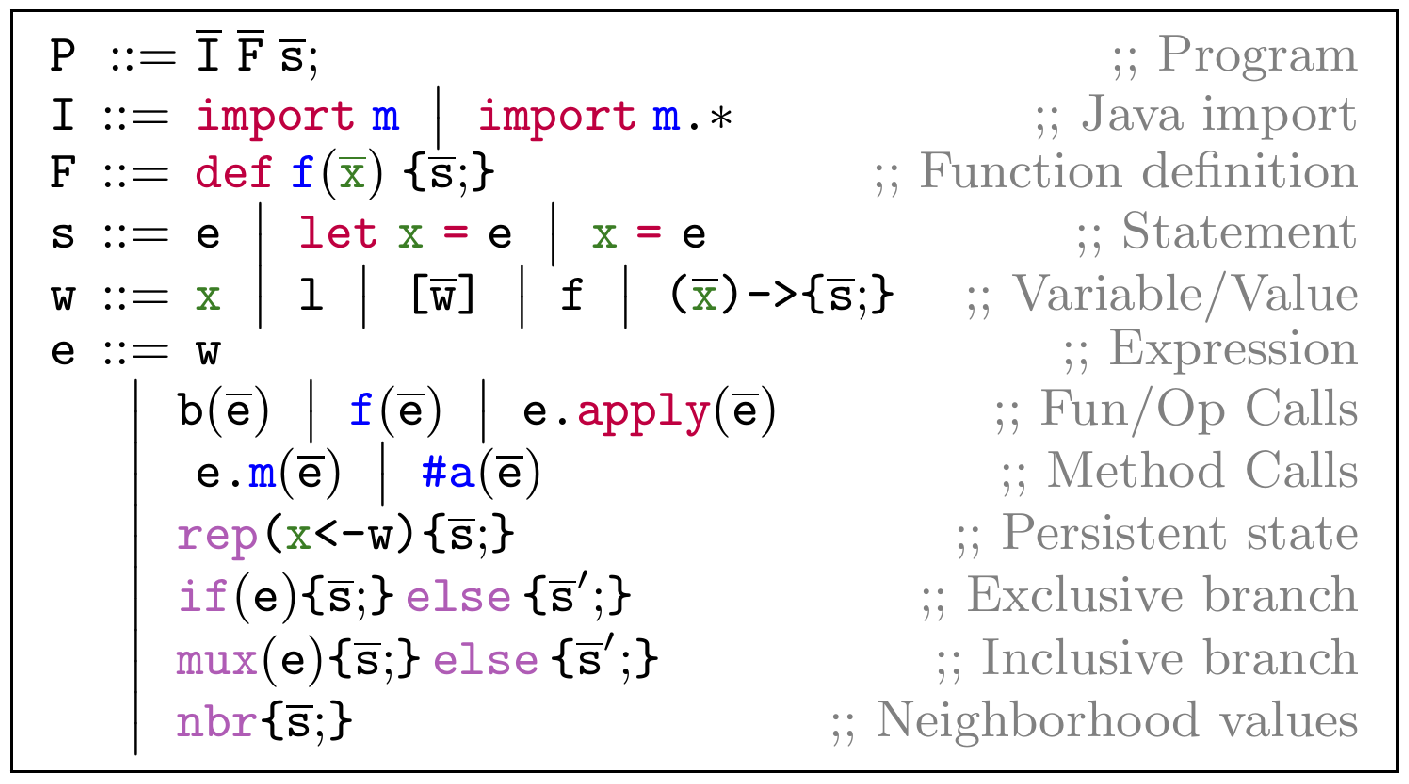
\includegraphics[width=.8\linewidth]{figures/protelis-syntax.png}
    \caption{Protelis abstract syntax}
    \label{fig:protelis-syntax}
\end{figure}

\subsubsection{Example: Rendezvous at a Mass Event}

In large public events, it can be challenging to meet with companions due to crowded areas, inaccessible rendezvous points, or difficulty in accessing cloud-based services.

Utilizing peer-to-peer geometric calculations across a network of devices to compute a \textit{rendezvous}\footnote{A meeting at an agreed time and place.} route is the proposed solution to the problem. The solution is demonstrated in a simulated city center environment (\Cref{fig:protelis-example-map}), using London as an example, with devices distributed randomly across the city streets. Each device has a communication range, and the goal is for two individuals (represented by their devices) to meet at a specific location.

The implementation (\Cref{lst:protelis-example}) involves injecting the environment of the devices with properties representing their owners (e.g., "Alice" and "Bob"). The algorithm measures the distance to one of the participants, creates a potential field, and builds an optimal path from the other participant, descending the distance potential field to reach the first participant at zero distance. The algorithm utilizes two main functions: \texttt{distanceTo} and \texttt{descend}. \texttt{distanceTo} measures the distance to one of the participants. Given a device and a potential field, \texttt{descend} builds a path of devices connecting the device with the source of the potential field. The algorithm elegantly compresses the entire process into a few lines of code, utilizing the \texttt{nbr} operator to exchange required information without explicitly declaring any communication protocol.

As \Cref{fig:protelis-example-map} shows, the simulation rapidly identifies a chain of devices (represented by red dots) that marks a sequence of waypoints for both device owners to walk and meet in the middle. The algorithm dynamically adjusts the path if one of the device owners moves in a different direction, ensuring it continues to recommend the best path for rendezvous.

\lstinputlisting[float,label={lst:protelis-example},caption=Rendezvous implementation in Protelis]{listings/protelis-example.txt}

\begin{figure}
    \centering
    \begin{subfigure}[b]{.49\textwidth}
        \centering
        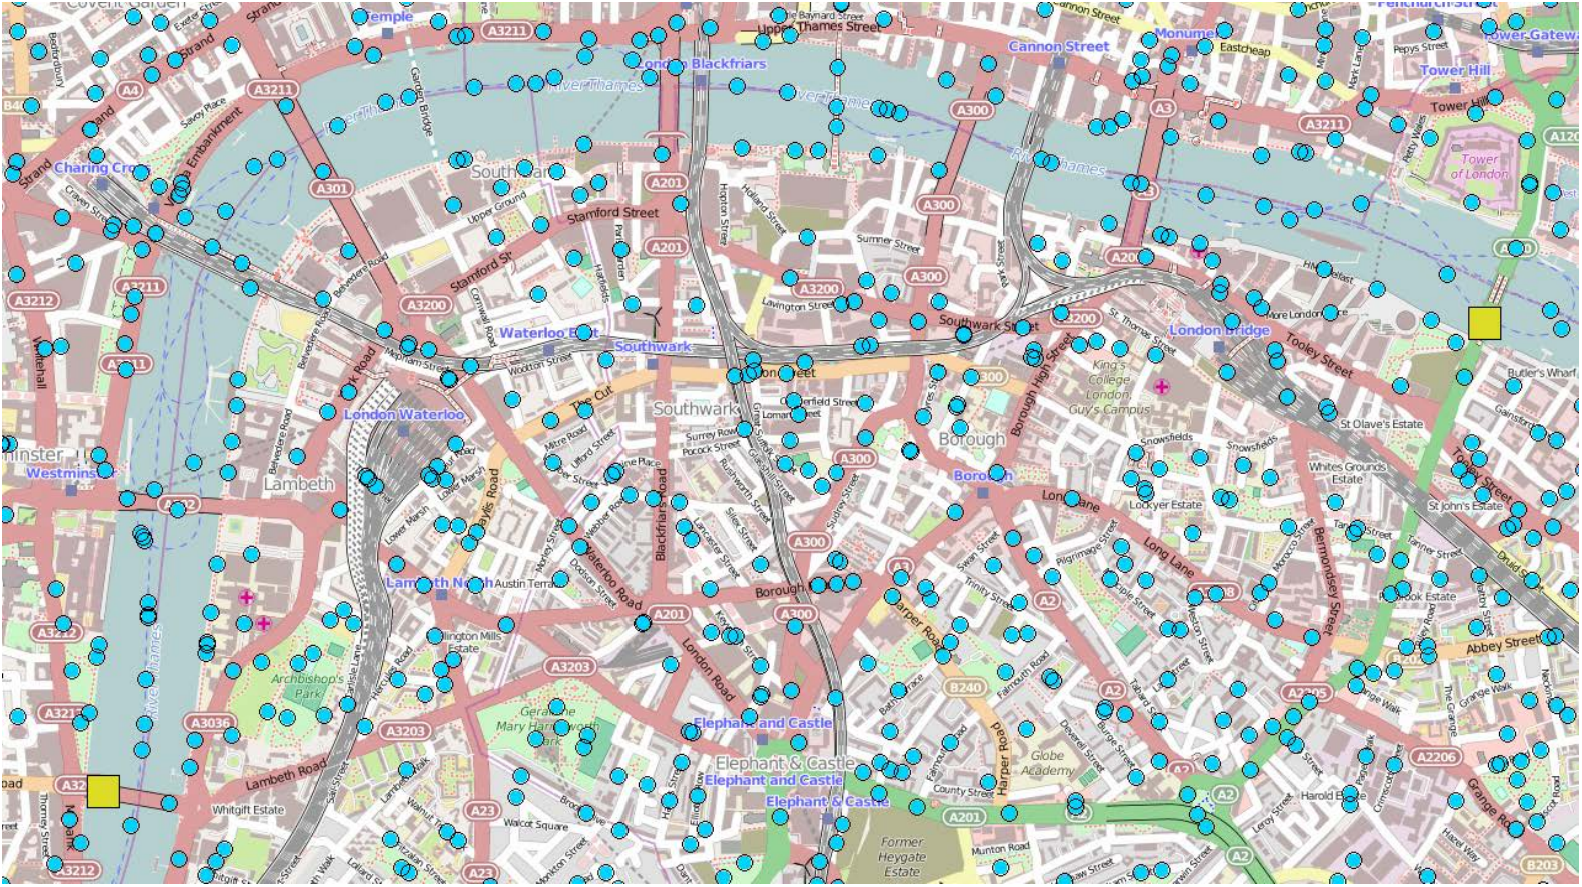
\includegraphics[width=\textwidth]{figures/protelis-example-a.png}
        \caption{Initial configuration.}
        \label{fig:protelis-example-a}
    \end{subfigure}
    \hfill
    \begin{subfigure}[b]{.49\textwidth}
        \centering
        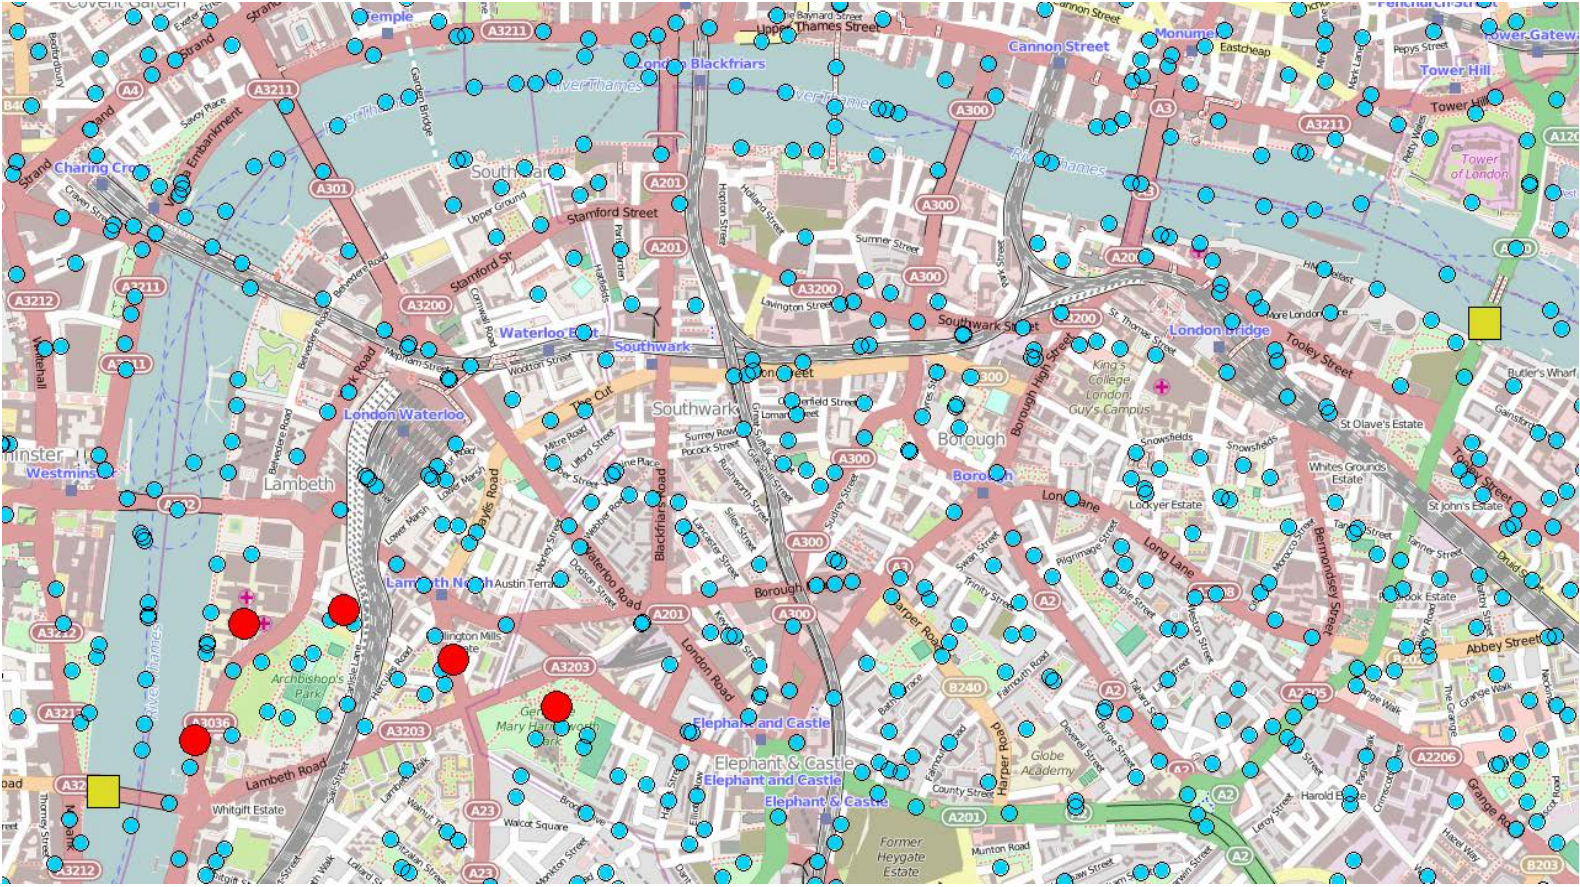
\includegraphics[width=\textwidth]{figures/protelis-example-b.png}
        \caption{Path begins to form.}
        \label{fig:protelis-example-b}
    \end{subfigure}
    \hfill
    \begin{subfigure}[b]{.49\textwidth}
        \centering
        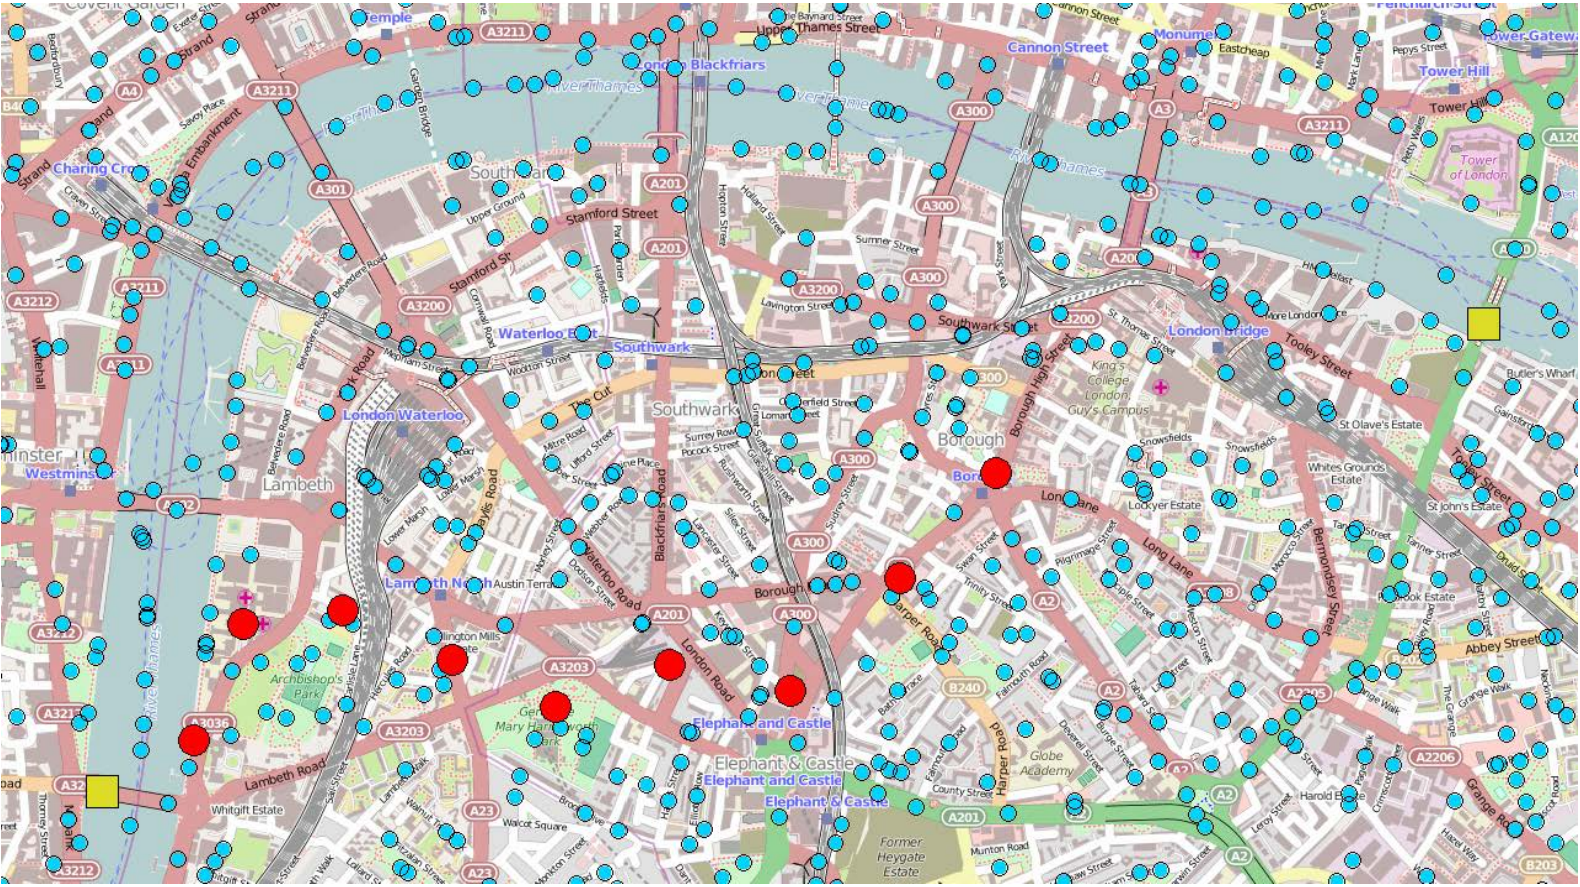
\includegraphics[width=\textwidth]{figures/protelis-example-c.png}
        \caption{Path continues to extend.}
        \label{fig:protelis-example-c}
    \end{subfigure}
    \hfill
    \begin{subfigure}[b]{.49\textwidth}
        \centering
        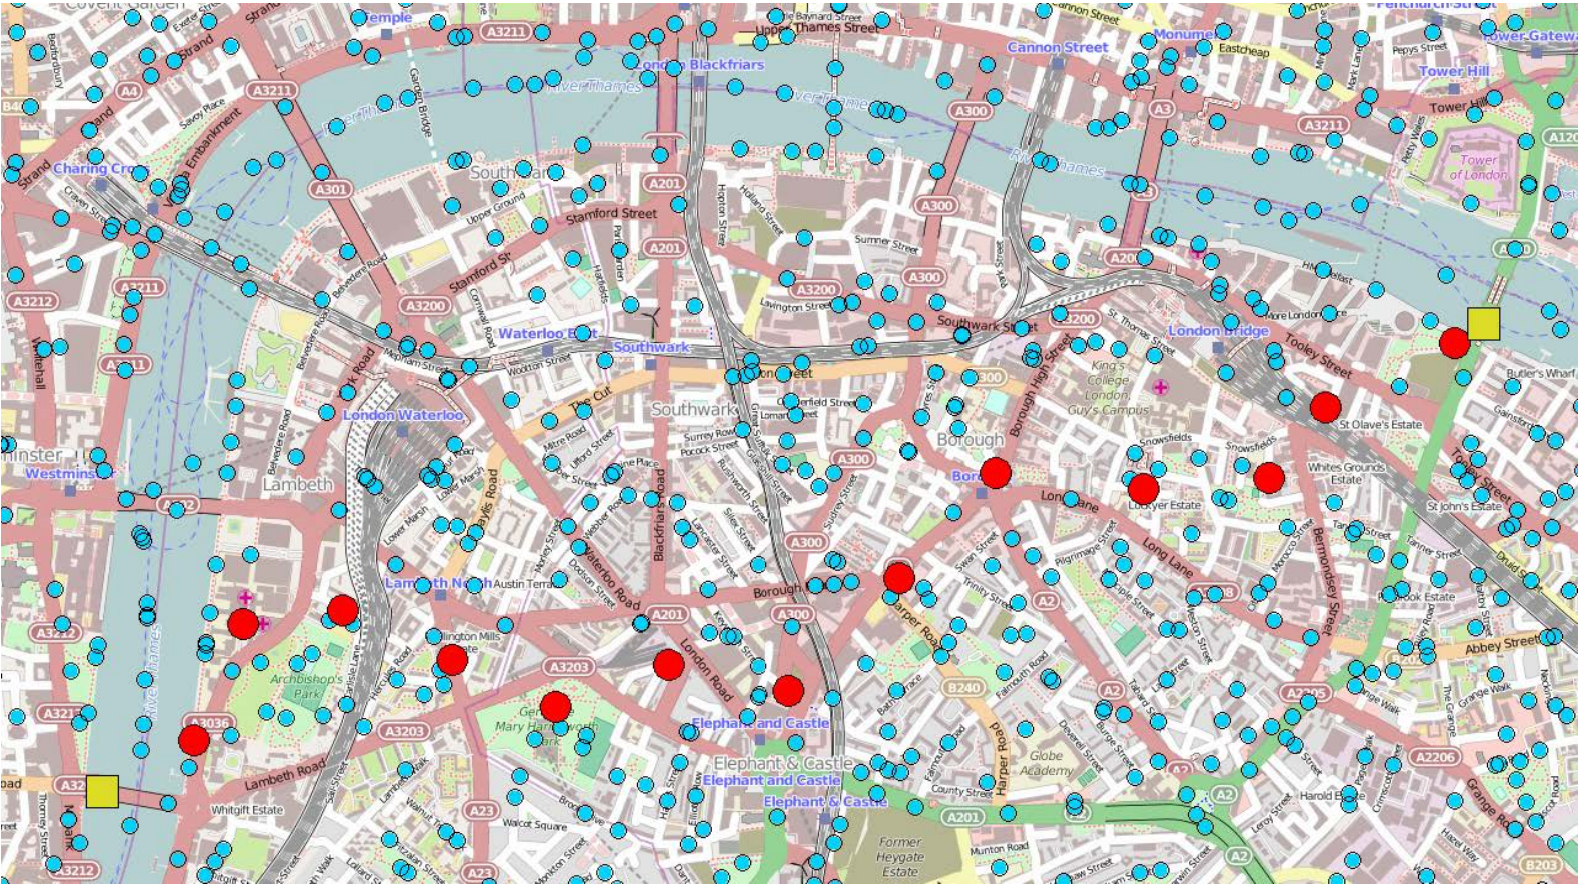
\includegraphics[width=\textwidth]{figures/protelis-example-d.png}
        \caption{Path computation complete.}
        \label{fig:protelis-example-d}
    \end{subfigure}
    \caption{Example of computing a rendezvous route for two people in a crowded urban environment.}
    \label{fig:protelis-example-map}
\end{figure}


\subsection{ScaFi}

ScaFi~\cite{Casadei2022} is a Scala-based library and framework designed for aggregate programming. It facilitates the development of distributed algorithms where computations are performed by individual devices in a network, and the results are aggregated across the network. The core concepts and constructs of ScaFi's API are outlined as follows:

\paragraph{Expression Evaluation}
An expression written using the ScaFi API is evaluated by each device once per computation round.

\paragraph{Fields}
Fields are represented as atomic values without any particular wrapper. They indicate the value of the field at the device performing the computation.

\paragraph{Neighboring Field}
The concept of ``neighboring field" from field calculus is not explicitly represented (not reified). Spatial computation (\texttt{nbr} and \texttt{nbrvar} constructs) is only available inside a special scope provided by the \texttt{foldhood} construct.

\paragraph{Export}
The export for each iteration is constructed by the ScaFi engine. It applies side effects to an internal data structure as the constructs are invoked, thereby constructing the evaluation tree.

\paragraph{Constructs}
The semantics of the constructs defined in ScaFi are described below:
\begin{itemize}
    \item \texttt{rep(init)(f)}: captures state evolution, starting from an \texttt{init} value that is updated each round through \texttt{f};
    \item \texttt{nbr(e)} captures communication, of the value computed from its \texttt{e} expression, with neighbors; it is used only inside the argument \texttt{expr} of \texttt{foldhood(init)(acc)(expr)}, which supports neighborhood data aggregation, through a standard “fold” of functional programming with initial value \texttt{init}, accumulator function \texttt{acc}, and the set of values to fold over obtained by evaluating expr against all neighbors;
    \item \texttt{branch(cond)(th)(el)} captures domain partitioning (space-time branching): essentially, the devices for which \texttt{cond} evaluates to \texttt{true} will run sub-computation \texttt{th}, while the others will run \texttt{el};
    \item \texttt{mid} is a built-in sensor providing the identifier of devices;
    \item \texttt{sense(sensorName)} abstracts access to local sensors;
    \item \texttt{nbrvar(sensorName)} abstracts access to “neighboring sensors” that behave similarly to \texttt{nbr} but are provided by the platform: i.e., such sensors provide a value for each neighbor.
\end{itemize}

\subsubsection{Gradient Implementation in ScaFi}

A \textit{(self-healing) gradient} is a distributed behavior that self-stabilizes, in each device of the distributed system, to a value denoting its minimum distance from the closest source node (for instance, computed by summing the neighbor-to-neighbor distances along the shortest path to the source), adapting to changes in the source set and distances. By following the neighbors of maximum decrease (resp. increase) of the gradient value, i.e., by descending (resp. ascending) the gradient, it is possible to implement efficient hop-by-hop information flows, that can be useful for data propagation and collection.

The implementation of a gradient using ScaFi is presented in \Cref{lst:scafi-gradient}. The following is a brief description of the program:
The gradient value at each node is dynamically evolved using \texttt{rep}. This is necessary to allow a node to share its previous gradient value with neighbors. The default value is \texttt{Double.PositiveInfinity} since by default a node is at an infinite distance from a source (since it may not be reachable in general). The \texttt{mux(c)(th)(el)} evaluates its expression \texttt{th} and \texttt{el} and then uses the Boolean condition \texttt{c} to select either the former (when \texttt{c} is true) or the latter (when \texttt{c} is false).
If a node is a source (i.e., if sensing the Boolean sensor \texttt{source} returns \texttt{true}), then its gradient value is \texttt{0} (by definition).
If a node is not a source, then will take as its gradient value the output of the expression \texttt{minHoodPlus(nbr\{distance\} + nbrRange)}.
\texttt{minHoodPlus(e)} is a variant of \texttt{foldhood} which does not consider the device itself when folding over the neighborhood. Namely, it selects the minimum value among those obtained by evaluating \texttt{e} against the neighbors. The argument of \texttt{minHoodPlus} is \texttt{nbr\{distance\} + nbrRange()}, which amounts to calculating, for each neighbor, the sum of the neighbor's most recent gradient value and the corresponding distance to that neighbor (obtained by neighboring sensor \texttt{nbrRange}, which is \texttt{nbrvar[Double]("nbrRange")}).

\lstinputlisting[float,label={lst:scafi-gradient},language=scala,caption=Implementation of gradient in ScaFi]{listings/scafi-gradient.scala}

\begin{figure}
    \centering
    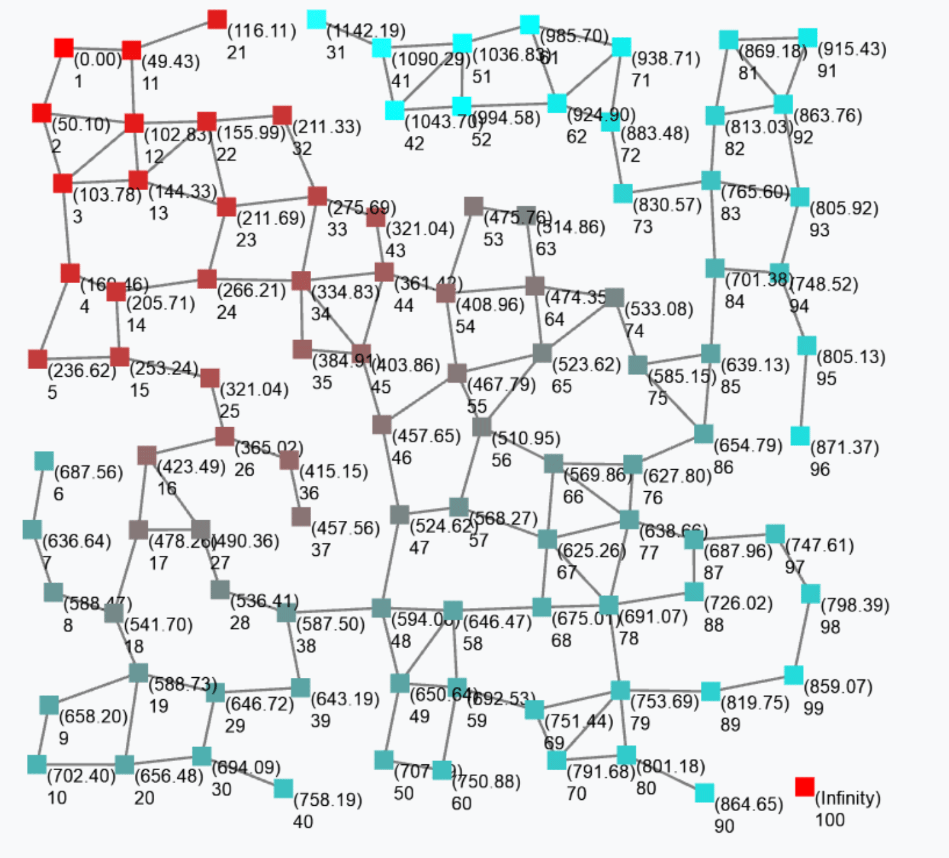
\includegraphics[width=\linewidth]{figures/scafi-gradient.png}
    \caption{A graphical representation of the gradient implementation in ScaFi after stabilization. Each device of the network is labeled with its distance from the source (in parenthesis) and its ID. The source device is the one with ID 1. Note that devices that are not connected to the source are considered to be at an infinite distance from it.}
    \label{fig:scafi-gradient}
\end{figure}

\subsection{FCPP}

FCPP~\cite{Audrito2020} is a C++14 library implementing Field Calculus and providing tools for distributed system simulation.

Its extensible component-based architecture allows customization for diverse application scenarios, such as Internet-of-Things (IoT) deployments, simulations, and self-organizing cloud applications. Users can add components tailored to specific functionalities, enhancing flexibility and applicability. The library incorporates compile-time optimizations and supports parallel execution, enabling efficient simulation of both systems and self-organizing cloud applications. Currently, FCPP focuses on distributed system simulations but already significantly reduces simulation costs, accelerating the development of new distributed algorithms. These features offer a path for a convenient extension to address previously ineffective scenarios:

Existing implementations often have high-performance requirements, unsuitable for resource-constrained microcontrollers. FCPP's lightweight nature makes it well-suited for these systems.

Self-organizing cloud applications necessitate fine-grained parallelism for scalability, and performance improvements directly translate to cost reduction. FCPP's support for parallelism caters to this need.

\subsubsection{Aggregate Program Example with FCPP}

The example function provided in \Cref{lst:fcpp-example} utilizes the Adaptive Bellman-Ford algorithm to estimate distances from devices where the \texttt{source} parameter is \texttt{true}. This function explicitly takes a \texttt{node} object as input, enabling access to its functionalities, including the \texttt{nbr\_dist()} method. This method returns a \texttt{field<double>} representing the estimated distances to neighboring nodes.

The \texttt{call\_point} parameter serves two purposes:

\begin{itemize}
    \item Updating the \texttt{node.stack\_trace} (shared functionality across all aggregate functions, as noted in the first line).
    \item Facilitating the aggregation of function calls (e.g., \texttt{nbr} and \texttt{min\_hood}) by providing an incrementing index.
\end{itemize}

\lstinputlisting[float,label={lst:fcpp-example},language=C++,caption=Implementation Adaptive Bellman Ford algorithm in FCPP]{listings/fcpp-example.cpp}

\subsection{Collektive}

Collektive\footnote{\url{https://github.com/Collektive/collektive}} provides the user with a \ac{dsl}, implemented in Kotlin, that allows to create aggregate programs transparently. It was designed with the following principles in mind: transparency, minimality and portability.

Transparency refers to the clear and concise information it provides about how the underlying system behaves, such as data processing, storage, and communication between nodes. Transparency helps to reduce complexity, making it easier to understand and maintain large and complex systems.

Collektive is designed with the fewest possible constructs and abstractions while still offering the required functionalities. This reduces the complexity of the system, making it easier to maintain and debug, and lowers the overhead associated with using the \ac{dsl}, which is particularly important for systems that require high performance and scalability.

Portability refers to its ability to run on various platforms and environments, including different operating systems, cloud platforms, and hardware architectures. This enables systems built with the \ac{dsl} to be easily deployed and run in different environments, which is crucial for systems requiring deployment in multiple locations or scalability to meet changing demands.

Constructs implemented in Collektive are defined in \Cref{lst:collektive-constructs}, while the semantics are described below:

\begin{itemize}
    \item \texttt{exchange}~\cite{https://doi.org/10.4230/lipics.ecoop.2022.20}: manages the computation of values between neighbors in a specific context. It computes a \texttt{body} function starting from the \texttt{initial} value and the messages received from other neighbors, then sends the results from the evaluation to specific neighbors or everyone, it is contingent upon the origin of the calculated value, whether it was received from a neighbor or if it constituted the initial value. The result of this function is a field with as messages a map with as key the ID of the devices across the network and the result of the computation passed as relative local values.
    \item \texttt{exchanging}: Same behavior of \texttt{exchange} but this function can yield a \texttt{Field} of \texttt{Return} value.
    \item \texttt{repeat}: Iteratively updates the value computing the \texttt{transform} expression at each device using the last computed value or the \texttt{initial}.
    \item \texttt{repeating}: Iteratively updates the value computing the \texttt{transform} expression from a \texttt{YieldingContext} at each device using the last computed value or the \texttt{initial}.
\end{itemize}

\lstinputlisting[float,label={lst:collektive-constructs},language=kotlin,caption=Base constructs implemented in Collektive]{listings/collektive-constructs.kt}

\subsubsection{Example of Gradient in Collektive}

In the \Cref{lst:collektive-gradient}, the implementation of the gradient in Collektive is presented. In this case, it is used a construct that is not strictly part of the field calculus but extends it; it is the \texttt{share} construct~\cite{https://doi.org/10.48550/arxiv.1910.02874}. \texttt{share} captures the space-time nature of field computation through observation of neighbors' values, starting from an \texttt{initial} value, it reduces to a single local value given a \texttt{transform} function and updating and sharing to neighbors of a local variable.

\lstinputlisting[float,label={lst:collektive-gradient},language=kotlin,caption=Gradient implementation in Collektive]{listings/collektive-gradient.kt}

\subsection{FRASP}
\label{section:frasp}

As said in \Cref{subsection:reactive-and-proactive-models}, aggregate computing makes use of a round-based execution model, that can be defined as proactive. This approach is simple to reason about but limited in terms of flexibility in scheduling and management of sub-activities (and response to contextual changes). In~\cite{Casadei2023} is proposed a reactive self-organization programming approach, called FRASP, that enables the decoupling of the program logic from the scheduling of its sub-activities. This model maintains the same expressiveness and benefits of aggregate programming while enabling significant improvements in terms of scheduling controllability, flexibility in the sensing/actuation model, and execution efficiency.

\subsubsection{Reactive Model}
\label{subsubsection:reactive-model}
FRASP is based on the functional reactive programming (FRP) paradigm and considers \textit{continuous time}, $Time$ = $\{ t \in \mathbb{R} \, | \, t \geq 0 \}$. Time-varying values are called \textit{cells} and may be conceptually modeled by generic functions of type $Cell$ $a$: $Time \rightarrow a$. Then, \textit{streams} are discrete-time values and may be modeled by generic functions of type $Stream$ $a$: $[Time] \rightarrow [a]$, namely, mapping a sequence of (increasing) sample times to a sequence of corresponding values. While cells model state, streams model state changes.

\subsubsection{Abstractions and Primitives}
\label{subsubsection:abstractions-and-primitives}

One of the main differences between the proactive and reactive models is that the latter allows the self-organizing collective computation to be expressed as a graph of reactive sub-computations. Each sub-computation is called \textit{flow} and represents it programmatically through type \texttt{Flow[T]}, where \texttt{T} is the type of the output of the wrapped computation. A \texttt{Flow} is essentially a function that takes a \texttt{Context} and returns a cell of \texttt{Export}s, possibly depending on the exports of other \texttt{Flow}s, recursively.

The details of the syntax and semantics of FRASP are discussed in detail in Section III of~\cite{Casadei2023} while in this section they are presented in a simplified manner:

\begin{itemize}
    \item \texttt{constant(e)} returns a constant flow that always evaluates to the argument that has been passed;
    \item \texttt{sensor(name)} returns the flow of values produced by the sensor with the given \texttt{name};
    \item \texttt{mid()} returns the constant flow of the device ID;
    \item \texttt{mux(c)\{t\}\{e\}} is an expression that returns a flow with the same output of flow \texttt{t} when the Boolean flow \texttt{c} is true and the output of flow \texttt{e} when \texttt{c} is false;
    \item \texttt{nbr(f)} handles communication with neighbors in both directions at once, it takes a flow \texttt{f} as a parameter;
    \item \texttt{branch(c)\{t\}\{e\}} evaluates and returns the value of expression \texttt{t} when \texttt{c} evaluates to true. This enables a form of distributed branching, where devices that happen to execute \texttt{t} will not interact with those that executed \texttt{e} (and vice versa);
    \item \texttt{loop(init,ft)} evolves a piece of state (initially, \texttt{init}) by applying function \texttt{ft} mapping the previous state's flow to the next state's flow.
\end{itemize}

\subsubsection{Gradient Implementation in FRASP}

\Cref{lst:frasp-gradient} provides a representation of a gradient in FRASP. The function takes the Boolean \texttt{src} flow as input, denoting whether the executing node is the source of the gradient or not. The external \texttt{loop} is used to progressively evolve the current gradient value \texttt{distance} starting from an infinite value (as, initially, devices do not know whether a source is reachable). Internally to the loop, \texttt{mux} is used to select one of two values: if the node is a source, then its gradient value is \texttt{0} (base case); otherwise, the gradient should be the minimum value among the neighbors' gradient values augmented by the distance (\texttt{nbrRange}) from that very neighbor. Construct \texttt{liftTwice} is used to combine (using the sum: \_+\_) the two flows \texttt{nbrRange} (distances to neighbors) and \texttt{nbr(distance)} (neighbors' gradient values).

\lstinputlisting[float,label={lst:frasp-gradient},language=scala,caption=Gradient implementation in FRASP]{listings/frasp-gradient.scala}

The reactive dataflow graph in \Cref{fig:gradient-dependencies} corresponds to \Cref{lst:frasp-gradient}. \Cref{fig:gradient-dependencies} provides the local view of the computation for a single node (where the layers denote different semantic kinds of dependencies), whereas \Cref{fig:gradient-dependencies-distributed} shows the distributed dependency graph. The arrows denote dependencies. The dashed arrows denote dependencies based on platform-level scheduling and node interaction; for instance, a red block depends on changes corresponding to neighbors' red blocks and is communicated via message passing.

\begin{figure}
    \centering
    \begin{subfigure}[b]{\textwidth}
        \centering
        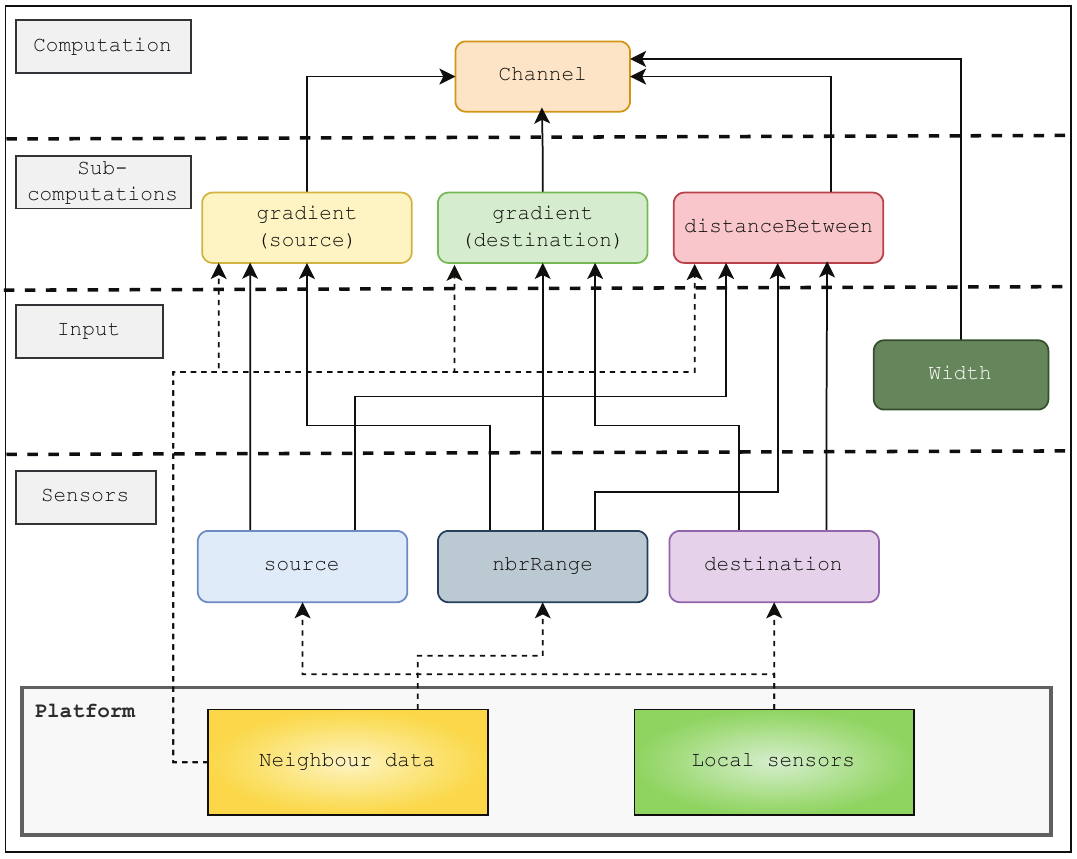
\includegraphics[width=\textwidth]{figures/gradient-dependencies.png}
        \caption{Node view.}
        \label{fig:gradient-dependencies}
    \end{subfigure}
    \hfill
    \begin{subfigure}[b]{\textwidth}
        \centering
        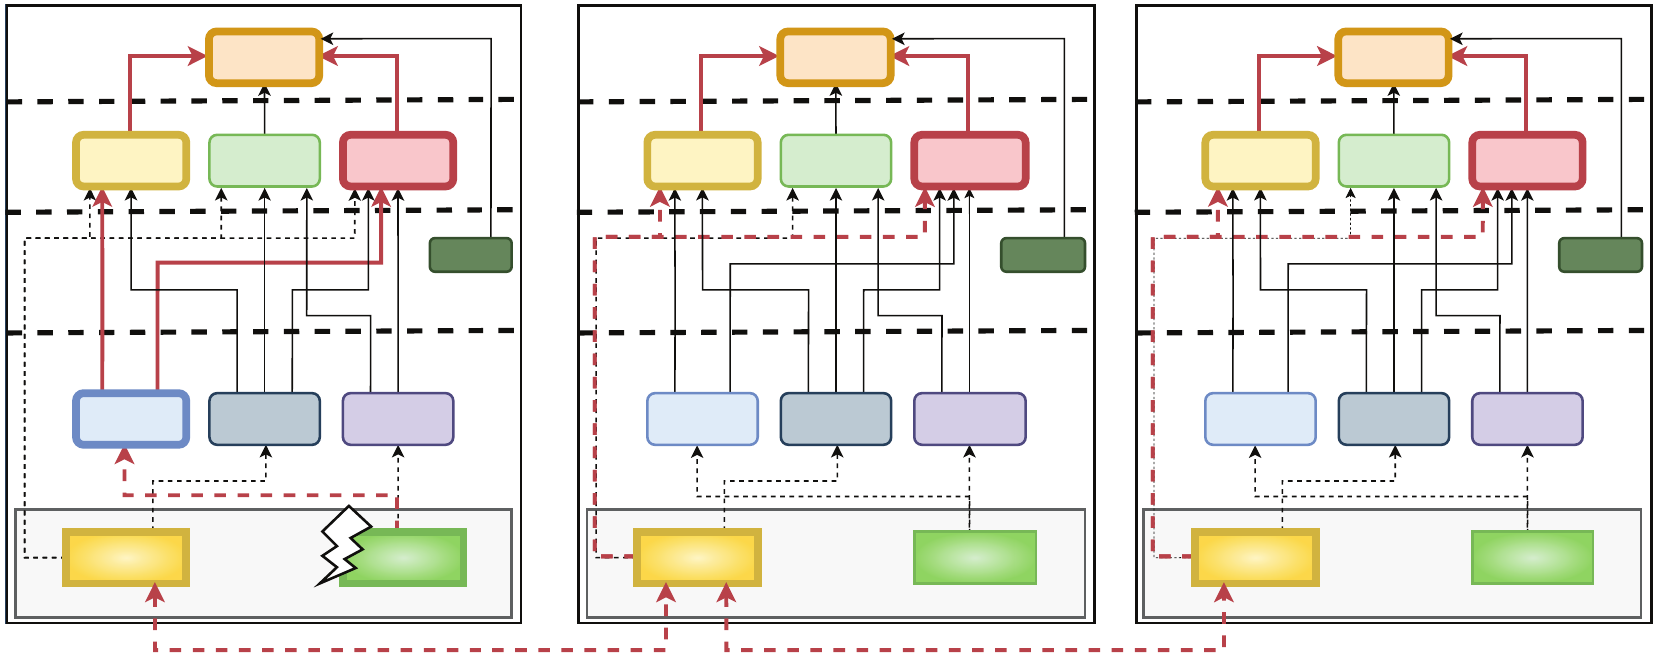
\includegraphics[width=\textwidth]{figures/gradient-dependencies-distributed.png}
        \caption{Distributed view (with neighbor dependencies).}
        \label{fig:gradient-dependencies-distributed}
    \end{subfigure}
    \caption{Dependencies between sub-computations in gradient program (\Cref{lst:frasp-gradient})}
\end{figure}

\section{Design of FRASP}
\label{section:design-of-frasp}

\subsection{Architecture}

The architecture of FRASP is shown in \Cref{fig:frasp-architecture}. The design is organized into three packages: \texttt{core}, which includes basic type definitions (\texttt{Core}) as well as the components for the \ac{dsl} (\texttt{Language} for primitives and \texttt{RichLanguage} for other built-ins) and its ``virtual machine" (\texttt{Semantics}), overall captured by an \texttt{Incarnation}; \texttt{frp}, which provides an interface to the FRP engine (\texttt{FrpEngine}), possibly also decoupling from the specific FRP library adopted, as well as extensions (\texttt{FrpExtensions}) useful for the definition of FRASP constructs; and simulation, which provides basic simulation support.

\begin{figure}
    \centering
    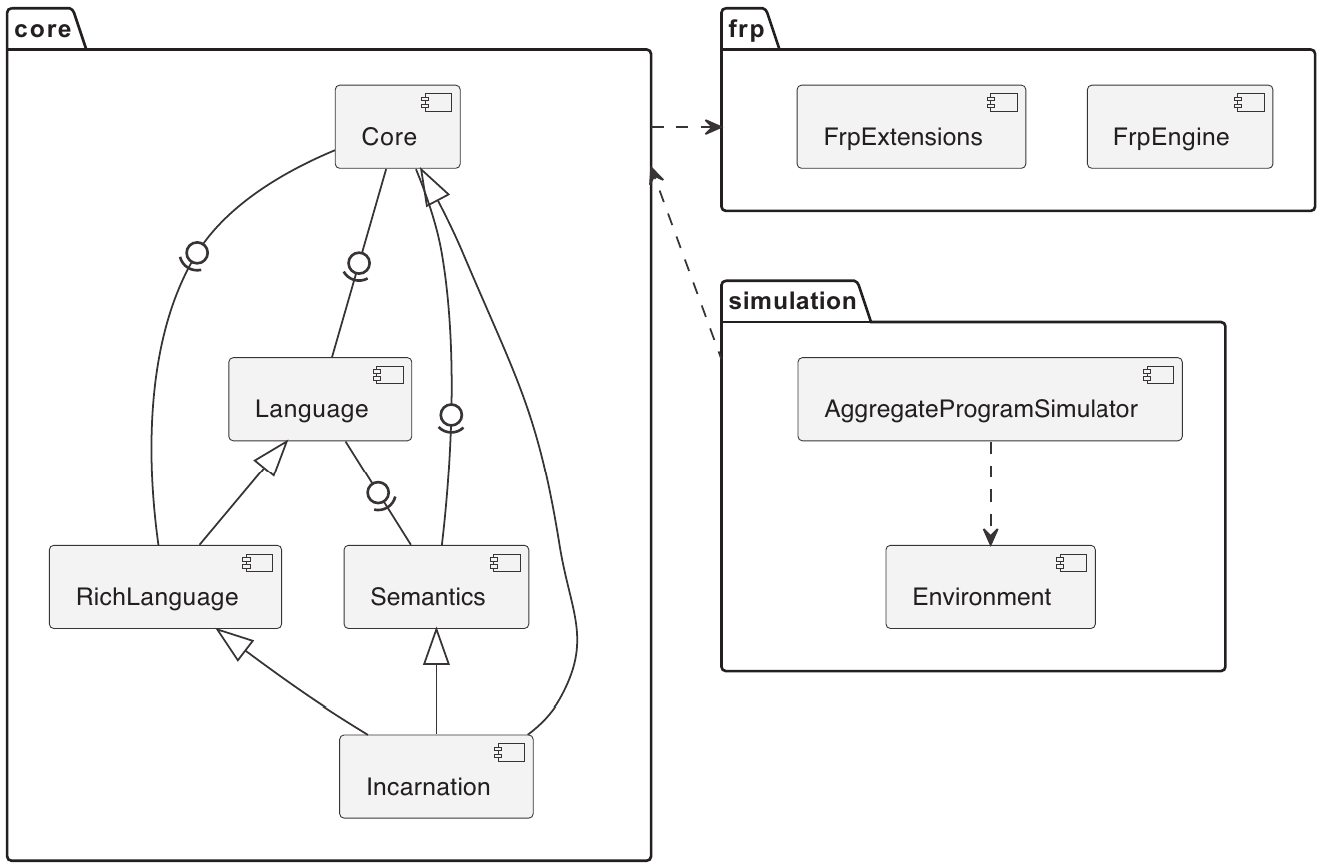
\includegraphics[width=\linewidth]{figures/FRASP-architecture.png}
    \caption{FRASP architecture.}
    \label{fig:frasp-architecture}
\end{figure}

\subsection{Detailed Design}

FRASP has been implemented in Scala, using Sodium as FRP library. Scala is well known for its suitability as a host for embedded \ac{dsl}s, and for aggregate computing embeddings as well. The design of the FRASP \ac{dsl} is
detailed in \Cref{fig:frasp-design}. Following the system/execution model described in \Cref{section:frasp}, the input and output of a (sub-)program are modeled through an interface \texttt{Context}, providing access to local sensor data and neighbor data; and an interface \texttt{Export}, capturing outputs and data that must be shared with neighbors. In particular, an \texttt{Export} is modeled as a tree where each node is a \texttt{Slot} (corresponding to a particular language construct) with an associated value, and can be located through a path of slots—e.g., \texttt{S1/S2/S3} identifies a node in the export tree, where \texttt{S1} depends on \texttt{S2} which depends in turn on \texttt{S3} (so, a change in the output \texttt{S3} will cause the expression corresponding to \texttt{S2} to re-evaluate, and possibly \texttt{S1} in turn). \texttt{Flow} is the type of a reactive (sub-)computation, which takes a \texttt{Context} (providing its inputs), a \texttt{Seq[Slot]} as path (indicating its position in the export tree), and returns \texttt{Cell} (i.e. a time-varying value) of \texttt{Export}. Each \texttt{Language} construct returns a \texttt{Flow}: therefore, the constructs do not immediately run upon evaluation, but rather an executable, reactive object denoting a computation graph whose nodes will execute as a response to change (\Cref{fig:gradient-dependencies}). Access to neighbor-related data is mediated by a \texttt{NeighborField} abstraction, which is the same provided by constructs supporting interaction with neighbors, i.e., \texttt{nbr} and \texttt{nbrSensor} 

\begin{figure}
    \centering
    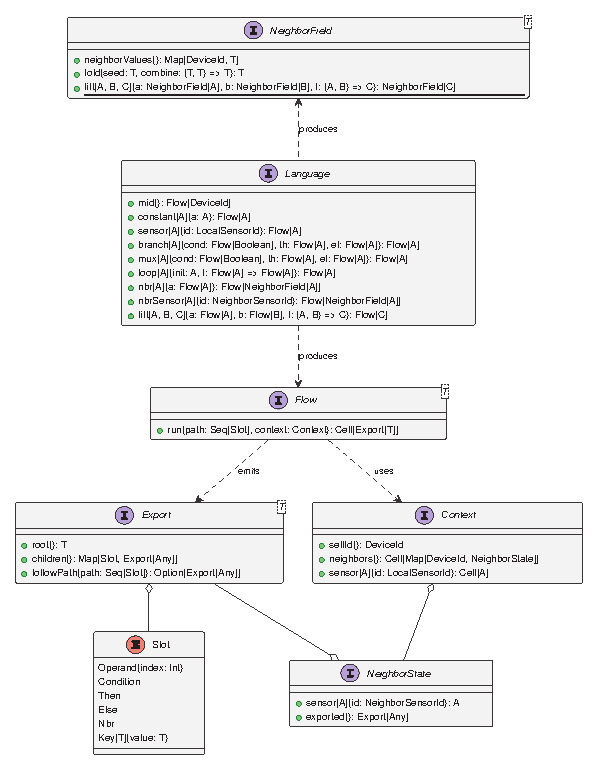
\includegraphics[width=\linewidth]{figures/FRASP-design.pdf}
    \caption{Detailed design of FRASP.}
    \label{fig:frasp-design}
\end{figure}

\section{Design of Collektive}
\label{section:design-of-collektive}

\subsection{Architecture}

Collektive has been developed as a Gradle project composed of three different submodules. The cited submodules are:

\begin{itemize}
    \item \texttt{plugin}, that is divided into two submodules:
    \begin{itemize}
        \item \texttt{gradle-plugin}: the necessary plugin used by a gradle project to include the compiler plugin.
        \item \texttt{compiler-plugin}: the compiler plugin is used to modify the data structure which is responsible for keeping track of the stack at runtime. For each aggregate function and branch construct, the stack data structure is updated to allow alignment whenever necessary.
    \end{itemize}
    \item \texttt{dsl}: the actual DSL implementation in Kotlin Multiplatform, where the logic is implemented and that exposes the operators of the aggregate computing.
    \item \texttt{alchemist-incarnation-collektive}: Allows to integrate Collektive simulations in the Alchemist~\cite{Pianini2013} simulator.
\end{itemize}

\subsection{Detailed Design}

The detailed design of Collektive is presented in \Cref{fig:collektive-design}. The \texttt{Collektive} class represents a device with a specific \texttt{localId} and a \texttt{Network} to manage incoming and outgoing messages, it takes a function to apply within the \texttt{AggregateContext}. \texttt{Collektive} implements two different execution strategies:

\begin{itemize}
    \item \texttt{cycle}: it applies once the aggregate function to the parameters of the device, then returns the result of the computation.
    \item \texttt{cycleWhile}: it applies the aggregate function to the parameters of the device while the condition is satisfied, then returns the result of the computation.
\end{itemize}

\texttt{cycle} and \texttt{cycleWhile} implicitly use the \texttt{aggregate} function, which is the entry point of the aggregate program. It computes an iteration of a device (\texttt{localId}), taking as parameters the previous \texttt{state}, the messages received from the neighbors and the \texttt{compute} with \texttt{AggregateContext} object receiver that provides the implementation of the aggregate constructs. Another version of the \texttt{aggregate} function computes an iteration of a device, over a \texttt{network} of devices, optionally from a previous state (\texttt{previousState}), running the \texttt{compute} aggregate program. The \texttt{aggregate} function returns an \texttt{AggregateResult}, which is the result of the aggregate computation. It represents the \texttt{localId} of the device, the \texttt{result} of the computation, the messages to send (\texttt{toSend}) to other devices and the new state (\texttt{newState}) of the device.

The interface \texttt{Aggregate} models the minimal set of aggregate operations and holds the \texttt{localId} of the device executing the aggregate program.

The \texttt{exchange} function manages the computation of values between neighbors in a specific context. It computes a \texttt{body} function starting from the \texttt{initial} value and the messages received from other neighbors, then sends the results from the evaluation to specific neighbors or to everyone, it is contingent upon the origin of the calculated value, whether it was received from a neighbor or if it constituted the initial value. The result of the \texttt{exchange} function is a \texttt{Field} with as messages a map with the ID of devices across the network as key and the result of the computation passed as relative local values.

The \texttt{alignOn} function is used for the alignment, it pushes in the stack the \texttt{pivot}, executes the \texttt{body} and pops the last element of the \texttt{Stack} after it is called, finally returns the \texttt{body}'s return element.

\texttt{AggregateContext} represents the context for managing aggregate computation. It represents the \texttt{localId} of the device, the messages received from the neighbors, and the previous state (\texttt{previousState}) of the device.

\begin{figure}
    \centering
    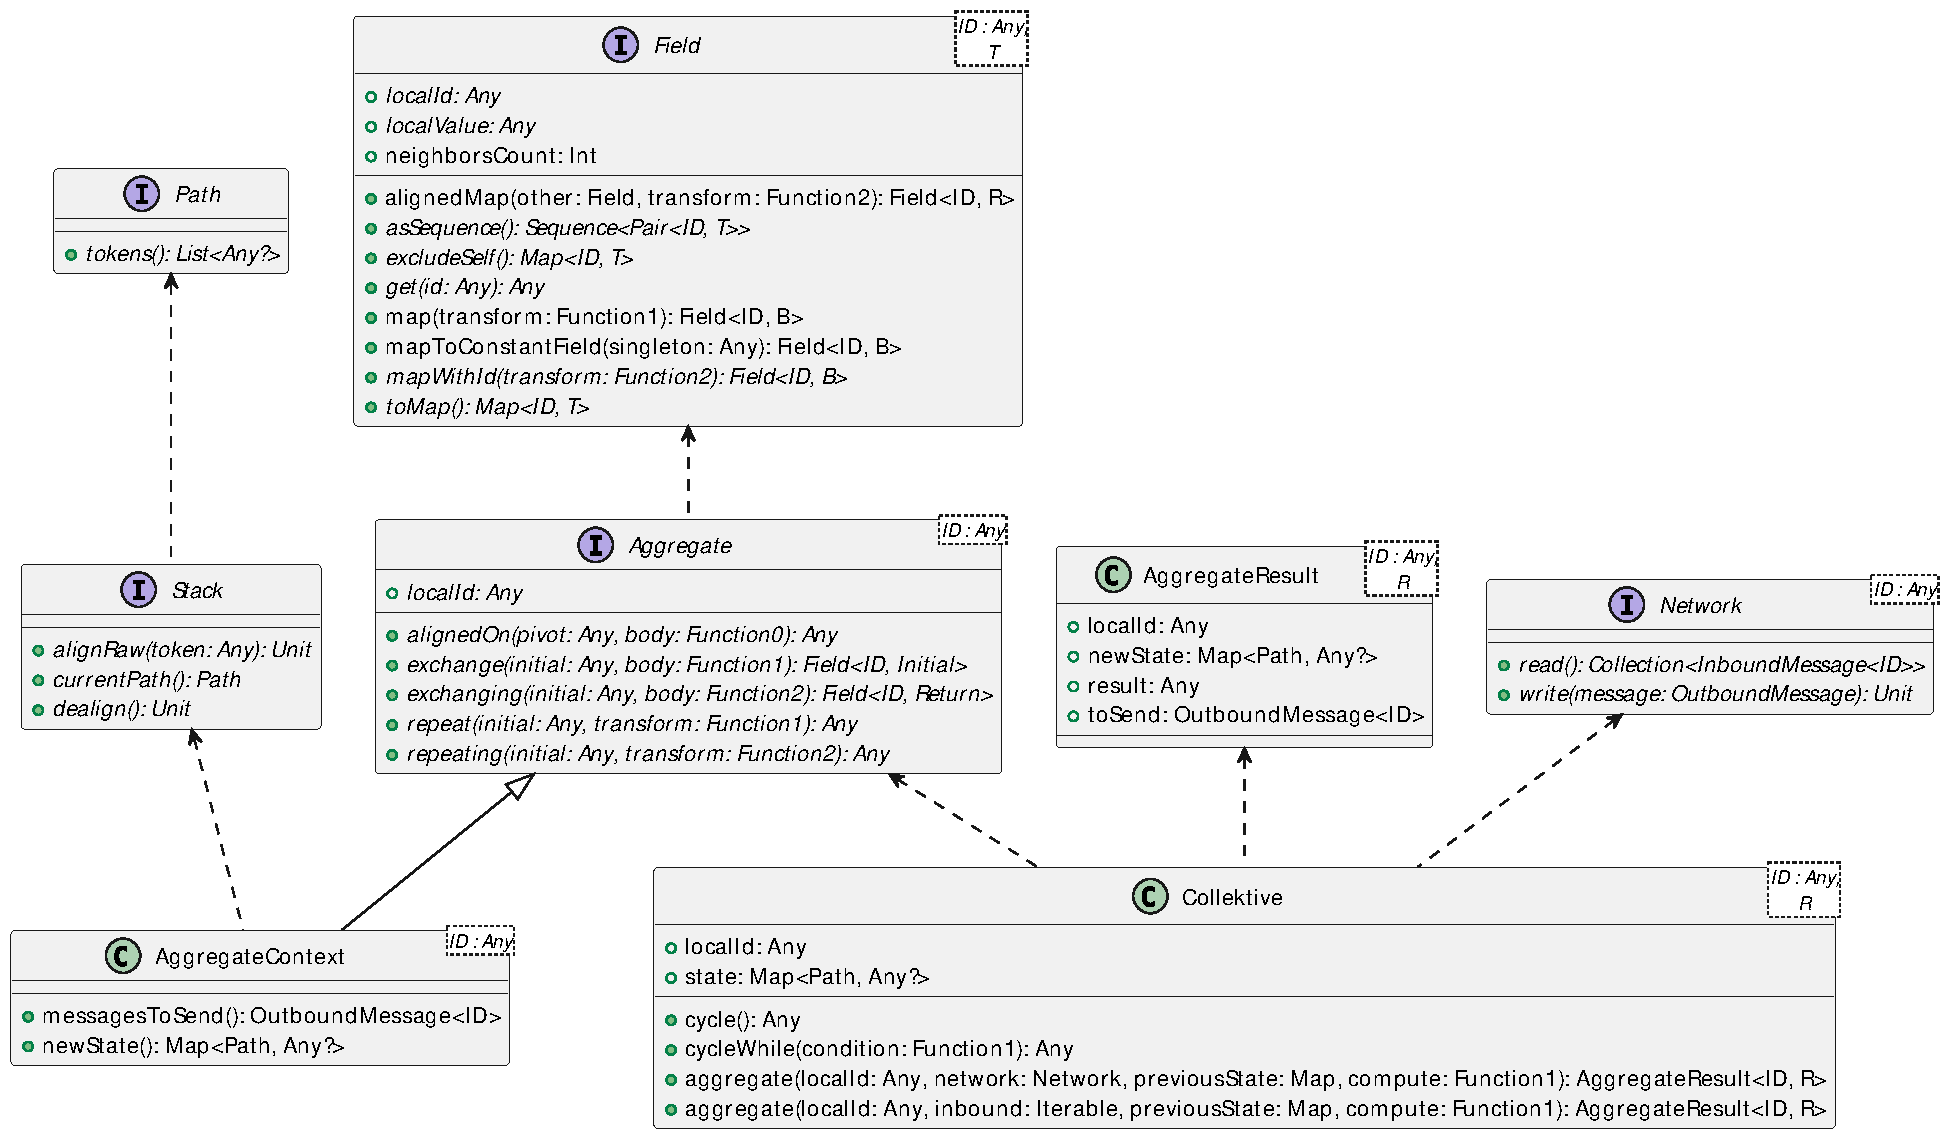
\includegraphics[width=\linewidth]{figures/collektive-design.pdf}
    \caption{Detailed design of Collektive DSL.}
    \label{fig:collektive-design}
\end{figure}

\subsection{Alignment Processing Strategy}

The alignment processing pursues the following strategy: in the first instance all the function definitions are visited and the ones involving aggregate computation will be subject to alignment processing. Then, for each candidate function, the plugin visits all the call sites in the body of the function and checks if the call has an aggregate reference or if it is involved in an aggregate computation. If so, the plugin will align the expression call. During the visiting of the function definition, branch conditions are also visited aligning only the branches that involve aggregate computation. If a branch body does not involve aggregate computation, the plugin will not align it. Aligning the branches in this way, by default all the branches follow the branch semantics of aggregate computing. The alignment strategy is formalized below:

\begin{enumerate}
    \item Each function definition exhibiting the following characteristics is the target of the alignment processing:
    \begin{itemize}
        \item The function has an \texttt{extensionReceiver} of type \texttt{Aggregate} or a subtype of it.
        \item The function has a \texttt{dispatchReceiver} of type \texttt{Aggregate} or a subtype of it.
        \item One or more of the function's parameters are of type \texttt{Aggregate} or a subtype of it.
    \end{itemize}
    \item For each candidate function, it aligns the call expressions having an aggregate reference or in-depth they involve an aggregate computation.
\end{enumerate}

\section{Integration of FRASP in Collektive}

Given the considerations regarding the proactive computational model made in \Cref{subsection:reactive-and-proactive-models} and the solution proposed in~\cite{Casadei2023} with the related results of the evaluations performed, it is decided to introduce the FRASP model in Collektive.
Analysis of the architectures of FRASP and Collektive, defined in \Cref{section:design-of-frasp} and \Cref{section:design-of-collektive}, respectively, reveals substantial differences in technology and design choices. This considerably complicates the process of integrating the reactive model into Collektive. The possible issues identified during the analysis are described in \Cref{subsection:integration-problems}.

\subsection{Integration Problems}
\label{subsection:integration-problems}

\subsubsection{Differences between Scala and Kotlin}
The Scala implementation of FRASP is extremely concise, even though it models several aspects of aggregate programming. In addition, the \ac{dsl} provided is particularly ergonomic, so the user can create aggregate programs easily and effectively. These characteristics of FRASP are due in part to the flexibility of Scala, which is given by the constructs that the language implements. The following are some Scala features that are used in FRASP but are not available by Kotlin:

\begin{itemize}
    \item \textbf{Given instances and using clauses}: Functional programming tends to express most dependencies as simple function parameterization. This is clean and powerful, but it sometimes leads to functions that take many parameters where the same value is passed over and over again in long call chains to many functions. Context parameters can help here since they enable the compiler to synthesize repetitive arguments instead of the programmer having to write them explicitly. Given instances define ``canonical" values of certain types that serve for synthesizing arguments to context parameters.
    \item \textbf{Traits and self-types}: Self-types are a way to declare that a trait must be mixed into another trait, even though it doesn't directly extend it. That makes the members of the dependency available without imports. A self-type is a way to narrow the type of \texttt{this} or another identifier that aliases \texttt{this}.
\end{itemize}

\subsubsection{Differences in Paths and Exports Management}

Typically, in aggregate computing implementations that respect the proactive model, paths are modeled as lists of tokens, while exports are represented by making use of maps that have the path as the key and the result of evaluating the sub-expression related to the path as the value.
In FRASP, these entities are represented in a completely different way; this is due to the need to properly model the dependencies of reactive sub-expressions. In particular, an export is modeled as a tree (using a specially defined data structure) where each node is a token with an associated value and can be located through a path of tokens.

\subsubsection{Diversity of Implemented Constructs}

FRASP implements a reactive version of the constructs defined by the field calculus, this allows a sub-expression to be automatically re-evaluated as one of the sub-expressions on which it depends changes. On the other hand, in addition to the field calculus constructs, Collektive implements a proactive version of \texttt{exchange} and \texttt{share}, so a reactive version of these two constructs must be provided.

\subsubsection{Divergences between Reactive and Proactive Models}

In the proactive model, at each round, the aggregate expression is reevaluated entirely, taking into account the following parameters passed in as input: previous state, neighbor messages, and sensors states. This behavior differs completely from the reactive model, where it is necessary to think in terms of dependencies between information flows instead of computational rounds. In other words, it is necessary to revisit the design of Collektive by modifying some aspects of it. The state, sensors, and messages of neighbors must be modeled as reactive entities, of which the values change over time; furthermore, in addition to modeling the aggregate constructs so that they are reactive, it is necessary to adequately define the dependencies between them and the context (state, sensors and neighbors messages) in which they are executed.

\subsection{Feasibility of Reactive Aggregate Programming in Kotlin}
\label{subsection:Feasibility-Reactive-Aggregate-Programming}

Even before addressing the problems presented in \Cref{subsection:integration-problems}, it is necessary to understand whether it is possible to create a Kotlin version of FRASP and, if so, analyze the similarities and differences with the model implemented in Scala, considering, in particular, the ergonomics of the \ac{dsl}. In this regard, an implementation of FRASP in Kotlin that makes use of the Flow library is proposed in the analysis phase to demonstrate the actual feasibility. Reactive values are modeled by making use of \texttt{StateFlow<T>}, whose behavior is similar to that of a \texttt{Cell}, described in \Cref{subsubsection:reactive-model}.

\Cref{fig:kotlin-distributed-frp-design} shows the design of the Kotlin version of FRASP. The implementation\footnote{\url{https://github.com/FilippoVissani/kotlin-distributed-frp}} includes only the subset of features from the Scala version of FRASP needed to demonstrate the feasibility of reactive aggregate programming. An aggregate expression is represented by a dedicated data structure (\texttt{AggregateExpression}) that produces a \texttt{StateFlow<ExportTree<T>>}, its behavior is similar to \texttt{Flow[T]} described in \Cref{subsubsection:abstractions-and-primitives}. The context of a device (\texttt{Context}) includes neighboring states, self ID and the state of the local sensors. Exports are modeled through a tree-like recursive data structure (\texttt{ExportTree}) holding data of type \texttt{T}. It exposes methods for accessing the \texttt{children} and the \texttt{root} element of a node and navigating through the tree using a \texttt{path}. \texttt{Semantics} implements field calculus functions (plus others useful in the reactive context) for constructing an \texttt{AggregateExpression}. These functions include \texttt{branch}, \texttt{constant}, \texttt{loop}, \texttt{mux}, \texttt{neighbor}, \texttt{selfID}, and \texttt{sense}. The enum \texttt{Slot} defines different types of tokens used within the \texttt{ExportTree} structure.

Given the proposed design in \Cref{fig:kotlin-distributed-frp-design} and its implementation, to demonstrate the ergonomics of the related \ac{dsl}, the implementation of the gradient is provided in \Cref{lst:kotlin-distributed-frp-gradient}. The results obtained demonstrate the actual feasibility of the solution, not only that, the \ac{dsl} appears ergonomic and easy to use, just like the one proposed in Scala (\Cref{lst:frasp-gradient}).

\begin{figure}
    \centering
    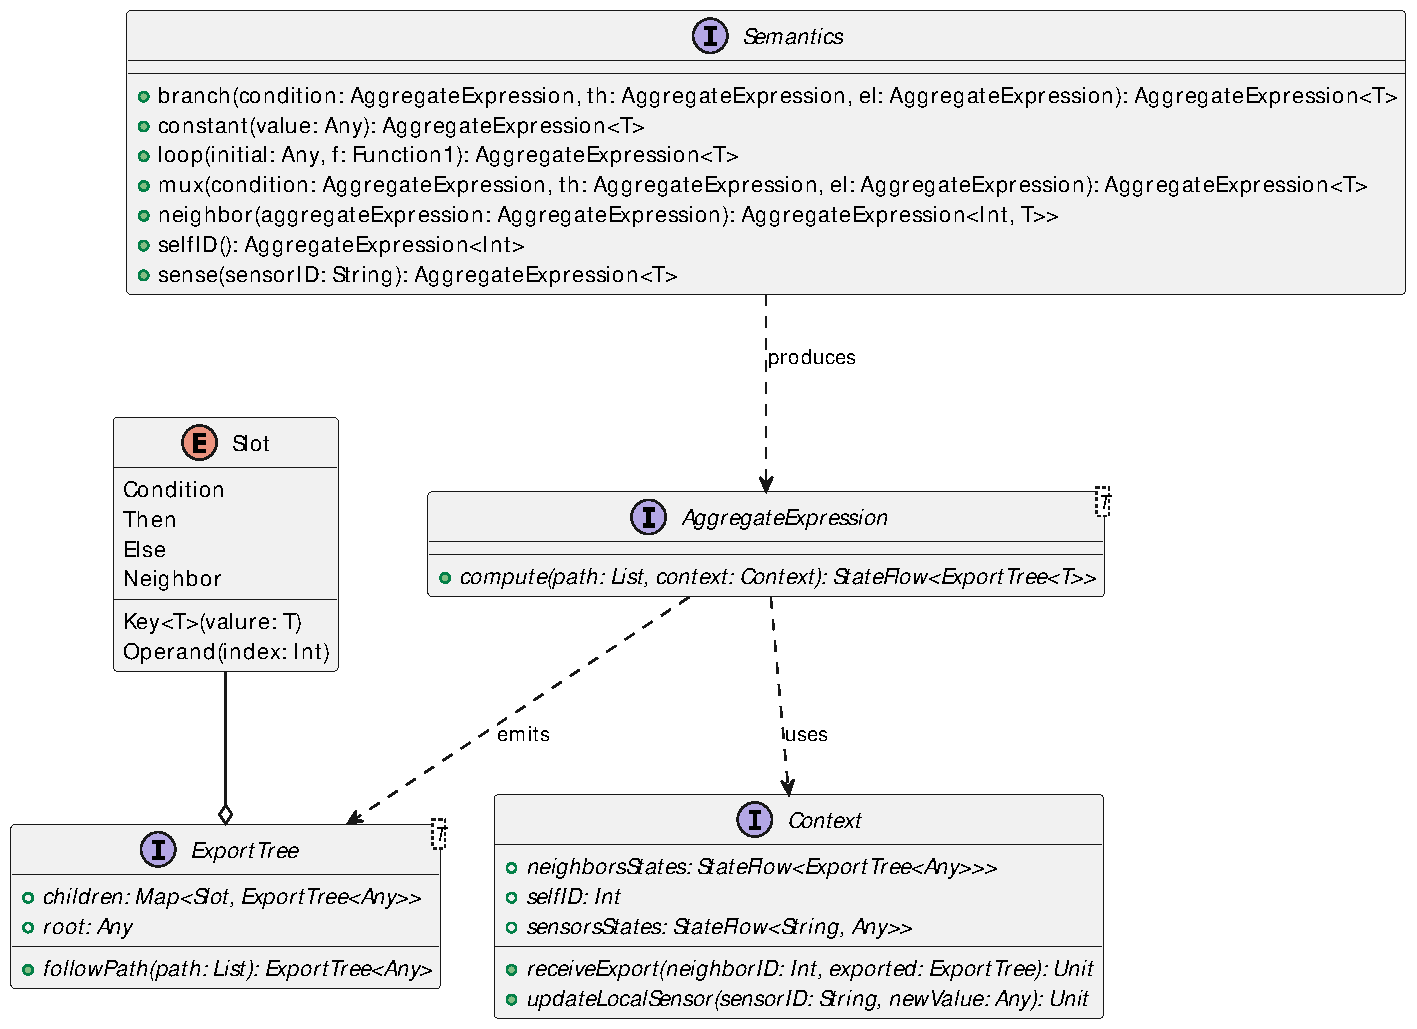
\includegraphics[width=\linewidth]{figures/kotlin-distributed-frp-design.pdf}
    \caption{Detailed design of Kotlin Distributed FRP.}
    \label{fig:kotlin-distributed-frp-design}
\end{figure}

\lstinputlisting[float,label={lst:kotlin-distributed-frp-gradient},language=kotlin,caption=Gradient implementation in Kotlin Distributed FRP]{listings/kotlin-distributed-frp-gradient.kt}

\subsection{Integration Solutions Identified}

The main goal is to introduce the reactive paradigm into Collektive, replacing it with the proactive one. At the same time, we want to make sure that the resulting DSL is ergonomic and thus it is easy for the user to understand and use it. It should be noted that, given the diversity of the two architectures, it is not possible to integrate FRASP directly into Collektive, so an intermediate solution must be identified.

Given the results obtained from the analysis reported in \Cref{subsection:Feasibility-Reactive-Aggregate-Programming} and taking into consideration the possible integration issues identified in \Cref{subsection:integration-problems}, we identify two possible solutions for integrating the reactive paradigm into Collektive:

\begin{itemize}
    \item \textbf{Model with reactive messages and sensors}: it consists of building the reactive model on top of the proactive one. This can be achieved by making the messages and sensors reactive; every time the value of one of these is changed the expression is re-evaluated entirely, executing a round. This solution has the advantage that the Collektive DSL remains identical to the current one. On the other hand, it is not possible to exploit the partial updates of the sub-expressions proposed in FRASP, this translates into lower efficiency.
    \item \textbf{Purely reactive model}: it consists of re-engineering all aggregate constructs and context definitions in Collektive to be reactive. In this case, important changes must be made to the current architecture of Collektive, making the implementation more complicated than the first solution. Furthermore, it is not possible to guarantee the ergonomics of the resulting DSL, as the definition of the aggregate constructs needs to be revised. The advantage of this solution is that, as in FRASP, it is possible to model the dependencies of the sub-expressions so that the latter can be updated only when necessary.
\end{itemize}
